\begin{figure}
\centering
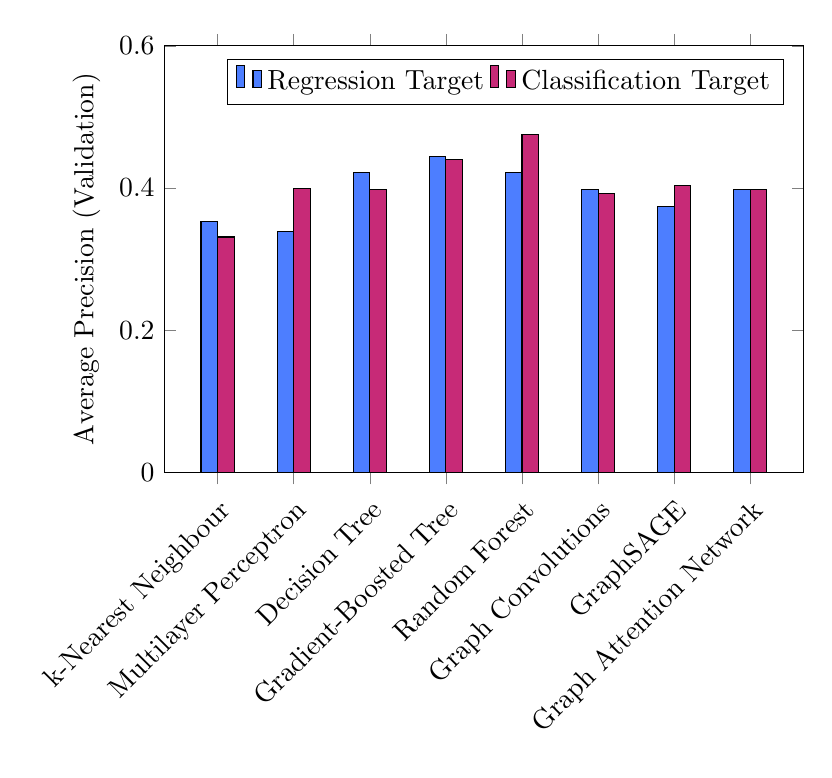
\begin{tikzpicture}
\definecolor{plotBlue}{RGB}{77,126,255}
\definecolor{plotPurple}{RGB}{97,75,202}
\definecolor{plotViolet}{RGB}{199,42,119}
\definecolor{plotOrange}{RGB}{245,80,27}
\definecolor{plotGreen}{RGB}{105,208,134}
\definecolor{plotBlack}{RGB}{255,255,255}
    \begin{axis}[
    ybar,
    bar width=6pt,
    width=0.8\textwidth,
    height=7cm,
    ymin=0,
    ymax=0.6,
    ylabel={Average Precision (Validation)},
    xtick=data,
    symbolic x coords={
        k-Nearest Neighbour,
        Multilayer Perceptron,
        Decision Tree,
        Gradient-Boosted Tree,
        Random Forest,
        Graph Convolutions,
        GraphSAGE,
        Graph Attention Network,
    },
    xticklabel style={rotate=45,anchor=north east},
    legend style={
        legend pos=north east,
        legend columns=2
    },
    ]

    \addplot[bar shift=-3pt,fill=plotBlue] coordinates {
        (Gradient-Boosted Tree, 0.4440352880707719)
        (Random Forest, 0.42126508450262135)
        (Decision Tree, 0.42126508450262135)
        (k-Nearest Neighbour, 0.3523807949098656)
        (Multilayer Perceptron, 0.33911571818438374)
        (Graph Convolutions, 0.3973)
        (GraphSAGE, 0.3734)
        (Graph Attention Network, 0.3973)
    };
    \addplot[bar shift=3pt,fill=plotViolet] coordinates {
        (Gradient-Boosted Tree, 0.44070016250479127)
        (Random Forest, 0.4747743632481278)
        (Decision Tree, 0.3983861433611597)
        (k-Nearest Neighbour, 0.3311685029371058)
        (Multilayer Perceptron, 0.39983671017473515)
        (Graph Convolutions, 0.3921)
        (GraphSAGE, 0.4030)
        (Graph Attention Network, 0.3984)
    };
    \legend{Regression Target,Classification Target}
    
    \end{axis}
\end{tikzpicture}
\caption{
    Average precision values of different models on validation data when classifying theories as problematic,
    for both regression (for lint frequency) and classification training targets.
}\label{fig:lint_freq_models_comp}
\end{figure}